\documentclass{beamer}


\usepackage[]{inputenc}
\usepackage[]{graphicx}
\usetheme{CambridgeUS}
\usefonttheme{serif}
\usepackage[french]{babel}
\usepackage{amsmath}
\usepackage[most]{tcolorbox}
\usepackage[]{float}
\usepackage{wrapfig}
\usepackage{interval}
\usepackage{amssymb}
\usepackage[]{tikz}
\usetikzlibrary{calc}
\usepackage{caption}
\usepackage{subcaption}\usepackage{chngcntr}
\usepackage{csvsimple}

\graphicspath{{./figures/}}

\newcommand{\textcircledd}[1]{%
	\tikz[baseline=(letter.base)] \node[draw, circle, inner sep=1pt] (letter) {#1};%
}

\setbeamertemplate{section in toc}[sections numbered]
\setbeamertemplate{subsection in toc}[subsections numbered]
\setbeamerfont{subsection in toc}{size=\scriptsize}
\setbeamerfont{section in toc}{size=\small}
\setbeamertemplate{enumerate items}[default]
\setbeamercolor{enumerate item}{fg=black}

\title[Les points de Lagrange]{Orbiter autour de... rien?\\{\normalsize Stabilité des points de Lagrange et cinématique dans leur voisinage}}
\author[ABDELOUAHAB Yannis]{\textbf{ABDELOUAHAB Yannis}, DUPLOUY Paul-Emmanuel}
\institute[21691]{SCEI 21691}
\date{Session 2026}


% Associé au package chngcntr pour numéroter les figures en 2.1.3 à la place de 17 par exemple
\counterwithin{figure}{subsection}
\renewcommand{\thefigure}{\thesubsection.\arabic{figure}}


\definecolor{darkred}{HTML}{7a2626}
\definecolor{captioncolor}{HTML}{660000}
\setbeamercolor{caption name}{fg=captioncolor}


% Compteur par ChatGPT
\setbeamertemplate{caption}[numbered]
\makeatletter
\@addtoreset{figure}{section}
\@addtoreset{figure}{subsection}
\makeatother
\renewcommand{\thefigure}{%
	\ifnum\value{subsection}=0
	\arabic{section}.\arabic{figure}%
	\else
	\arabic{section}.\arabic{subsection}.\arabic{figure}%
	\fi
}
\captionsetup[figure]{justification=centering}
% Fin du code par ChatGPT (fonctionne normalement bien)
\setbeamerfont{caption}{size=\scriptsize}

\setbeamertemplate{itemize item}[circle]
\setbeamertemplate{itemize subitem}[circle]
\setbeamertemplate{itemize subsubitem}[circle]
\setbeamercolor{itemize item}{fg=black}
\setbeamercolor{itemize subitem}{fg=black}
\setbeamercolor{itemize subsubitem}{fg=black}


% Pour faire les sources des photos
\newcommand{\photosources}[1]{%
	\begin{tikzpicture}[remember picture,overlay]
		\node[
		anchor=south west,
		yshift=0.28cm,
		font=\tiny,
		text=gray!110
		] at (current page.south west)
		{\textit{Source(s)} : #1};
	\end{tikzpicture}%
}

\newtcolorbox{importantresult}[1]{
	coltitle=darkred,
	title={#1},
	colback=red!2,
	colframe=darkred!20,
	boxrule=1pt,
	arc=.5mm
}

\definecolor{brown}{HTML}{663705}
\definecolor{lightbrown}{HTML}{996a39}
\newtcolorbox{mydefinition}[1]{
	coltitle=brown,
	title={Définition : #1},
	colback=lightbrown!2,
	colframe=brown!20,
	boxrule=1pt,
	arc=.5mm
}

\AtBeginSection[]
{
	\begin{frame}
		\frametitle{Sommaire}
		\tableofcontents[currentsection]
	\end{frame}
}


\begin{document}	
	
	
	\begin{frame}
		\titlepage
	\end{frame}
	
	
	
	
	\section{Objectif}
	\begin{frame}
		\frametitle{Introduction}
		\begin{figure}[h]
			\centering
			\begin{subfigure}[b]{0.2\textwidth}
				\centering
				\uncover<1->{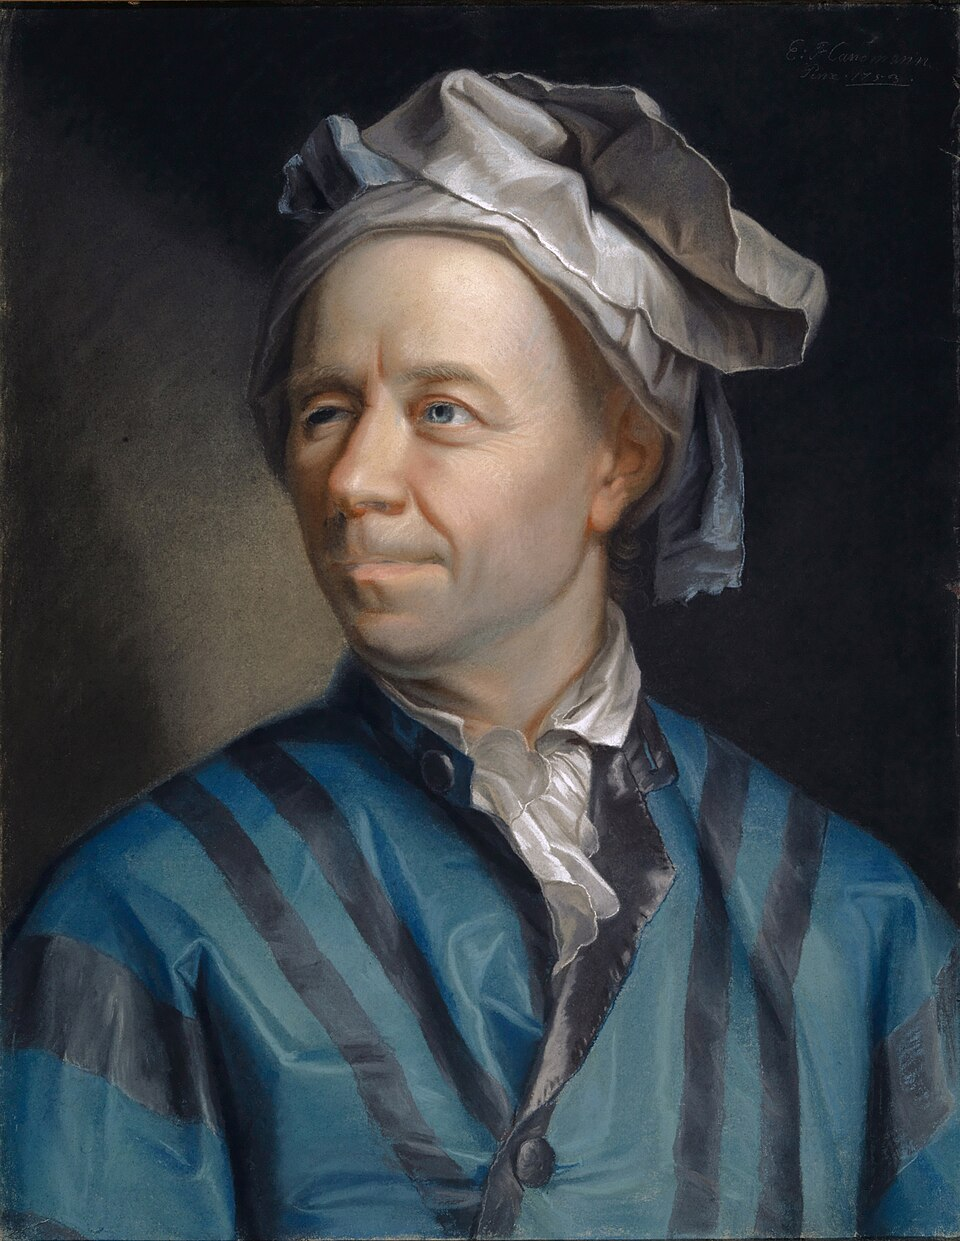
\includegraphics[width=\linewidth]{./euler_portrait.jpg}}
				\caption{Leonhard Euler}
				\label{fig:portrait de Euler}
			\end{subfigure}\hfill
			\begin{subfigure}[b]{0.23\textwidth}
				\centering
				\uncover<1->{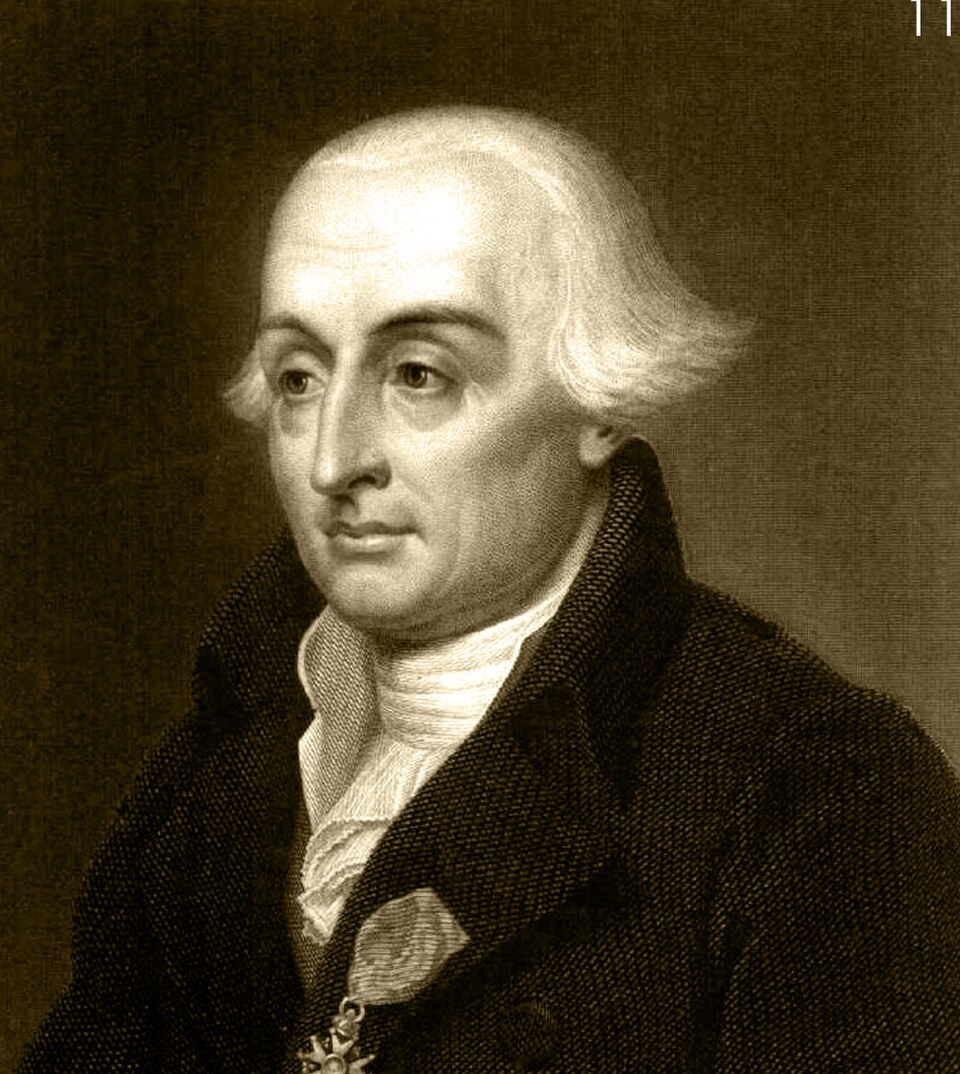
\includegraphics[width=\linewidth]{lagrange_portrait.jpg}}
				\caption{Joseph-Louis Lagrange}
				\label{fig:portrait de Lagrange}
			\end{subfigure}\hfill
			\begin{subfigure}[b]{0.45\textwidth}
				\centering
				\uncover<2->{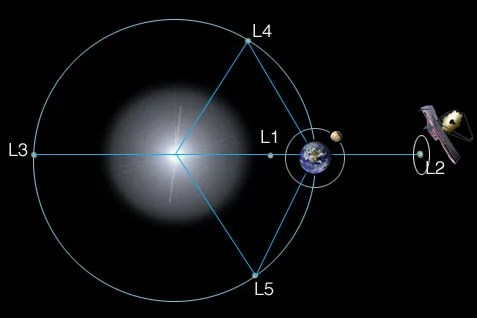
\includegraphics[width=\linewidth]{webb_orbit.png}}
				\uncover<2->{\caption{Orbite du James Webb Space Telescope}}
				\label{fig:orbite de JWST}
			\end{subfigure}
			\label{fig:firstfig}
			\caption{}
		\end{figure}

		\photosources{NASA \;|\; Wikimedia Commons}
	\end{frame}
	
	\begin{frame}
		\frametitle{Objectif}
		\textbf{Objectif :}
		\linebreak
		
		Comprendre en quoi les points de Lagrange $L_1$ et $L_2$ sont intéressants pour les missions spatiales d'observation, et leur utilité dans la création de trajectoires moins demandeuses en carburant.
	\end{frame}
	

	
	
	
	\section[Étude des points colinéaires]{Dynamique au voisinage des points d'équilibres colinéaires}
	
	\subsection{Définition du système, équations du mouvement}
	\begin{frame}
		\frametitle{Choix du référentiel}
		
		\begin{figure}
			\centering
			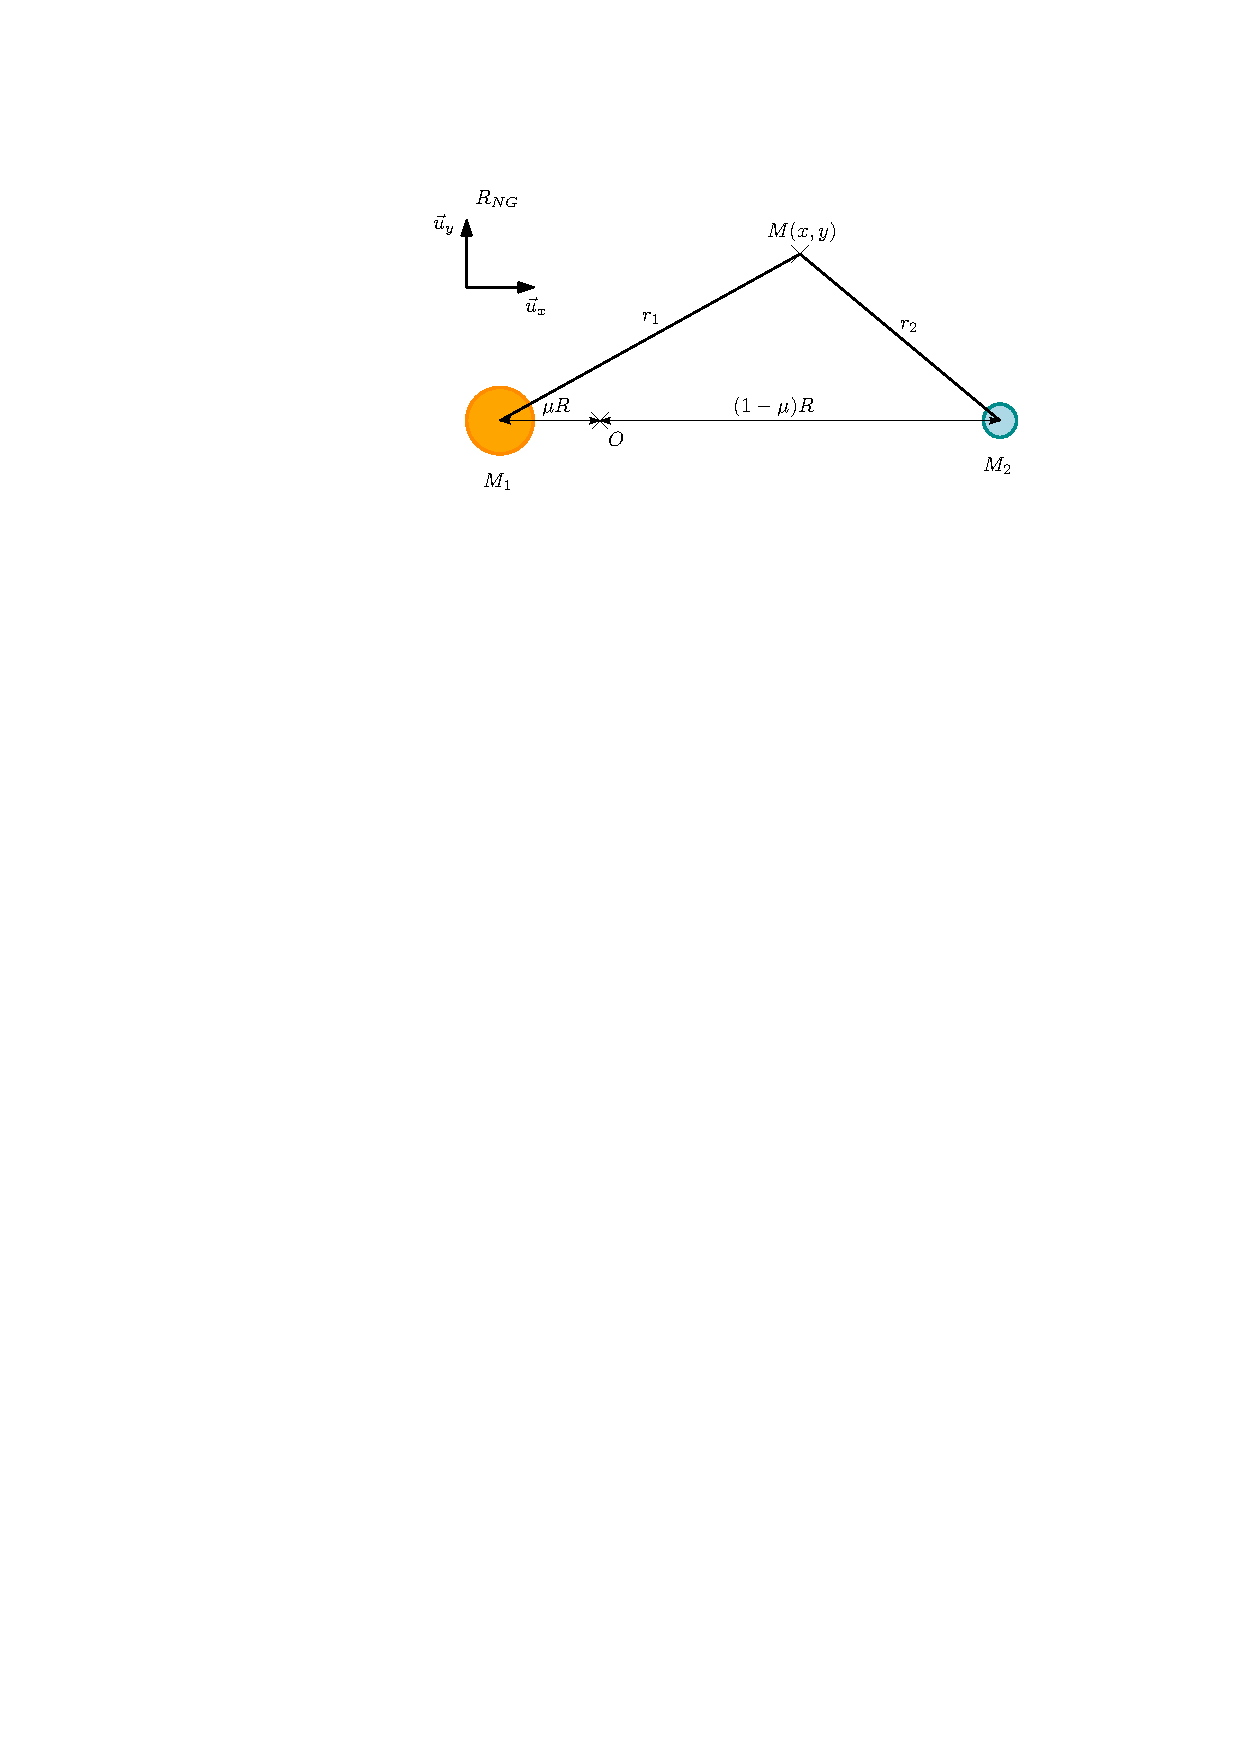
\includegraphics[width=0.7\linewidth]{ref_rng_diag.pdf}
			\caption{Plan $(O, \vec{u}_x, \vec{u_y})$ dans le référentiel barycentrique $R_{NG}$ en co-rotation avec le système Soleil–Terre.}
			\label{fig:schéma du référentiel de co-rotation avec la ligne M1-M2}
		\end{figure}
		{\footnotesize Avec $\mu := \frac{M_2}{M_1+M_2}$ le \textit{coefficient de masse} du système.}
		
	\end{frame}
	
	\begin{frame}
		\frametitle{Équations du mouvement}
		Les équations du mouvement dans le plan défini à la figure \ref{fig:schéma du référentiel de co-rotation avec la ligne M1-M2} sont :
		\begin{equation*}
			\label{eq du mvt}
			\begin{cases}
				\ddot{x} - 2\omega\dot{y} = - \frac{1}{m}\frac{\partial \bar{U}}{\partial x} \\
				\ddot{y} + 2\omega\dot{x} = - \frac{1}{m}\frac{\partial \bar{U}}{\partial y}
			\end{cases}
		\end{equation*}
		\pause
		et on a
		\begin{importantresult}{Expression du potentiel apparent}
			\begin{equation}
				\bar{U} = U(x,y) - \frac{1}{2}m\omega^2(x^2+y^2)
				\label{expression du potentiel apparent}
			\end{equation}
		\end{importantresult}
		{\small où $U(x,y) = \mathcal{E}_{p,1} + \mathcal{E}_{p,2}$ est la somme des énergies potentielles.}
	\end{frame}
	
	\begin{frame}
		\frametitle{Représentation du potentiel apparent}
		\begin{figure}
			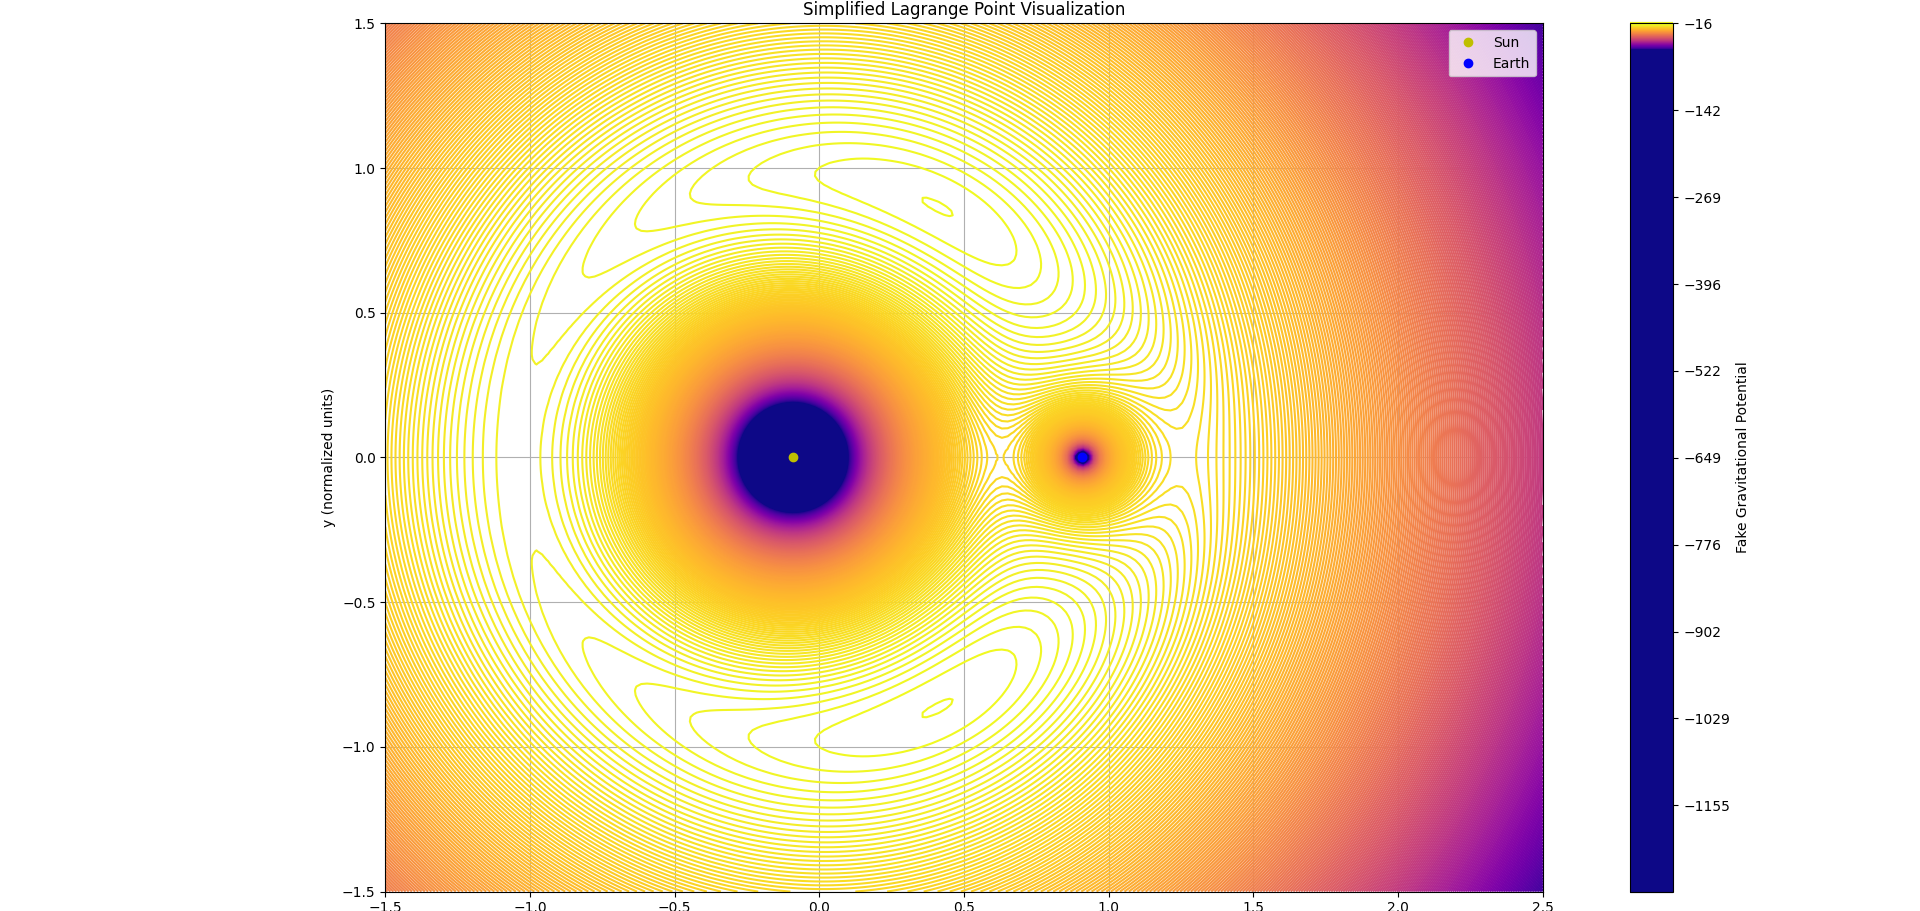
\includegraphics[width=1\linewidth]{potential_apparent_2D_moi.png}
			\caption{Tracé du potentiel apparent $\bar{U}$ en Python (cf. Annexe \ref{code python du tracé de potentiel apparent}) avec des grandeurs arbitraires.}
		\end{figure}
	\end{frame}
	
	\begin{frame}
		\frametitle{Représentation du potentiel apparent}
		\begin{figure}
			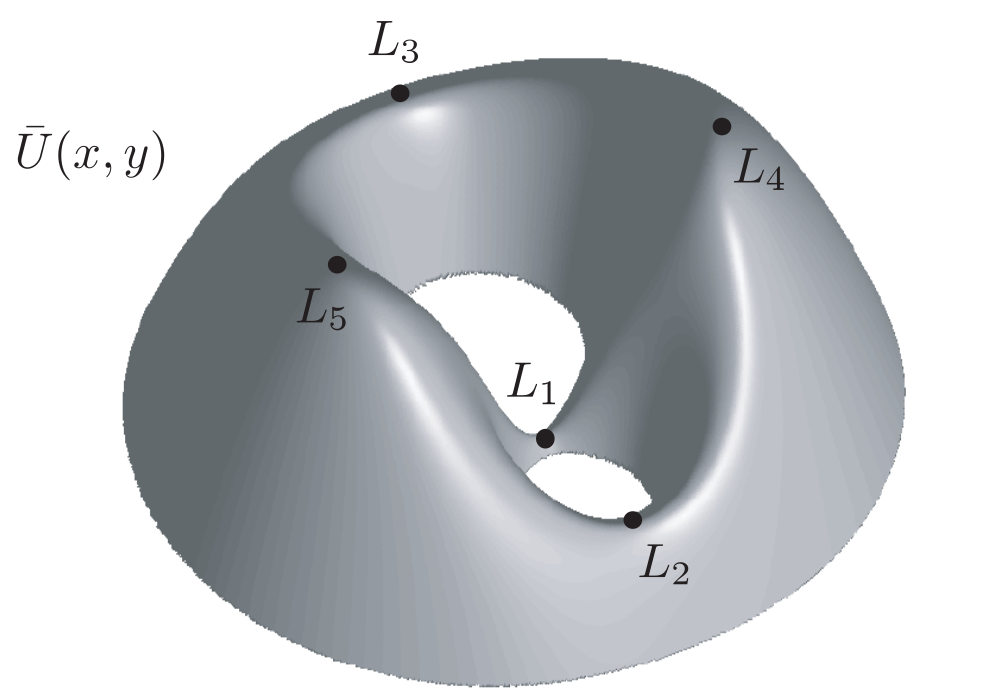
\includegraphics[width=0.7\linewidth]{potentiel_apparent_3D.png}
			\caption{Représentation 3D du potentiel apparent.}
		\end{figure}
		\photosources{Dynamical Systems, the Three-Body Problem
			and Space Mission Design}
	\end{frame}
	
	\subsection{Localisation des points d'équilibre}
	\begin{frame}
		\begin{importantresult}{Condition nécessaire d'équilibre :}
			\begin{equation}
				\label{condition nécessaire d'équilibre}
				\nabla \bar{U}(x,y) = \begin{bmatrix}
					\frac{\partial \bar{U}}{\partial x} (x,y) \\ 
					\frac{\partial \bar{U}}{\partial y} (x,y)
				\end{bmatrix} = 0
			\end{equation}
		\end{importantresult}
		
		\bigskip
		
		\pause
		
		\begin{columns}[T]
			\column{0.48\linewidth}
			\textbf{Cas $y=0$ :}
			\begin{figure}
				\centering
				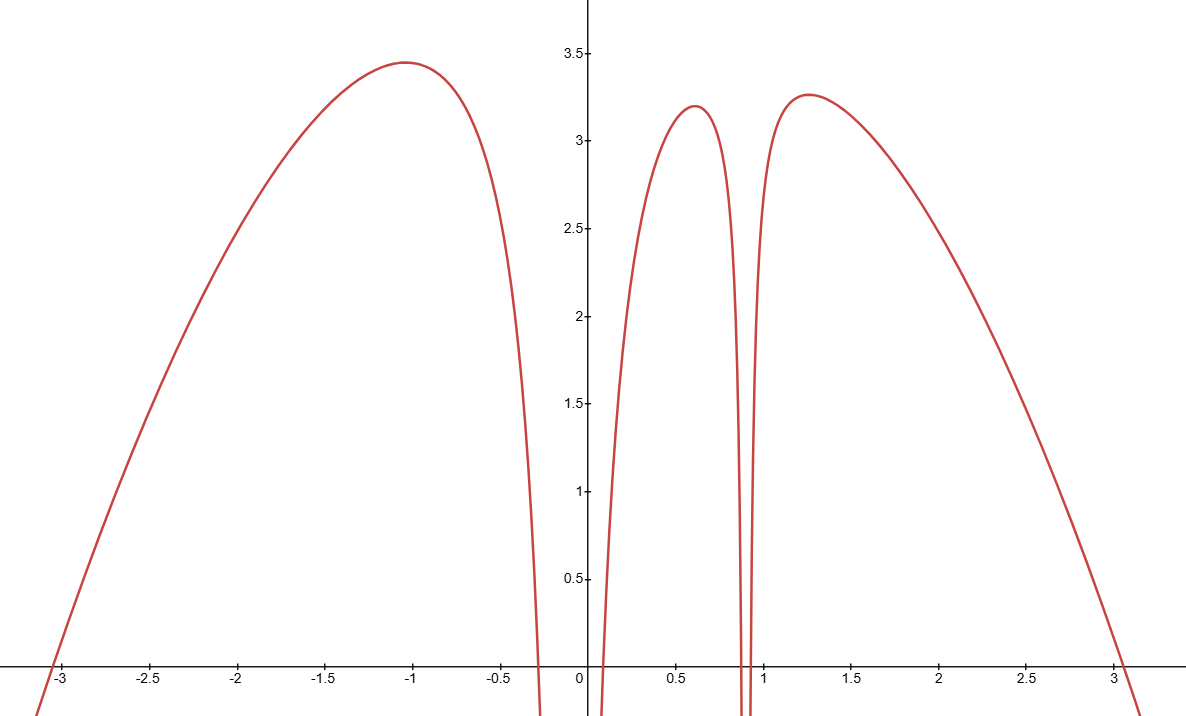
\includegraphics[width=0.8\textwidth]{graphe_potentiel_en_x.png}
				\caption{Tracé de $\bar{U}(\cdot, 0)$.}
			\end{figure}
			
			\column{0.04\textwidth}
			\centering
			\textcolor{gray!40}{\rule{0.2pt}{0.4\textheight}}
			
			\pause
			\column{0.48\linewidth}
			\textbf{Cas général :}
			
			{\small Si on suppose $y \neq 0$ alors on a la condition}
			\begin{equation*}
				r_1 = r_2 = R
			\end{equation*}
			{\small où $r_1$ et $r_2$ sont définis comme dans la figure \ref{fig:schéma du référentiel de co-rotation avec la ligne M1-M2}.}
		\end{columns}
	\end{frame}
	
	\begin{frame}
		\frametitle{Solutions à la condition (\ref{condition nécessaire d'équilibre})}
		\begin{figure}[H]
			\centering
			\label{tab:toutes_les_coord}
			\renewcommand{\arraystretch}{1.6}
			\begin{tabular}{|c|c|c|}
				\hline
				Point & Coordonnée en $x$ & Coordonnée en $y$
				\\ \hline
				L1 & $((1-\mu) - (\frac{\mu}{3})^{\frac{1}{3}})R$ & 0
				\\ \hline
				L2 & $((1-\mu) + (\frac{\mu}{3})^{\frac{1}{3}})R$ & 0
				\\ \hline
				L3 & $(-1-\frac{5\mu}{12})R$ & 0
				\\ \hline
				L4 & ($(\frac{1}{2}-\mu)R$) & $\frac{\sqrt{3}}{2}R$
				\\ \hline
				L5 & ($(\frac{1}{2}-\mu)R$) & $-\frac{\sqrt{3}}{2}R$
				\\ \hline
			\end{tabular}
			\caption{Coordonnées des points de Lagrange.}
		\end{figure}
	\end{frame}
	
	\begin{frame}
		\frametitle{Représentation des points de Lagrange}
		\begin{figure}
			\centering
			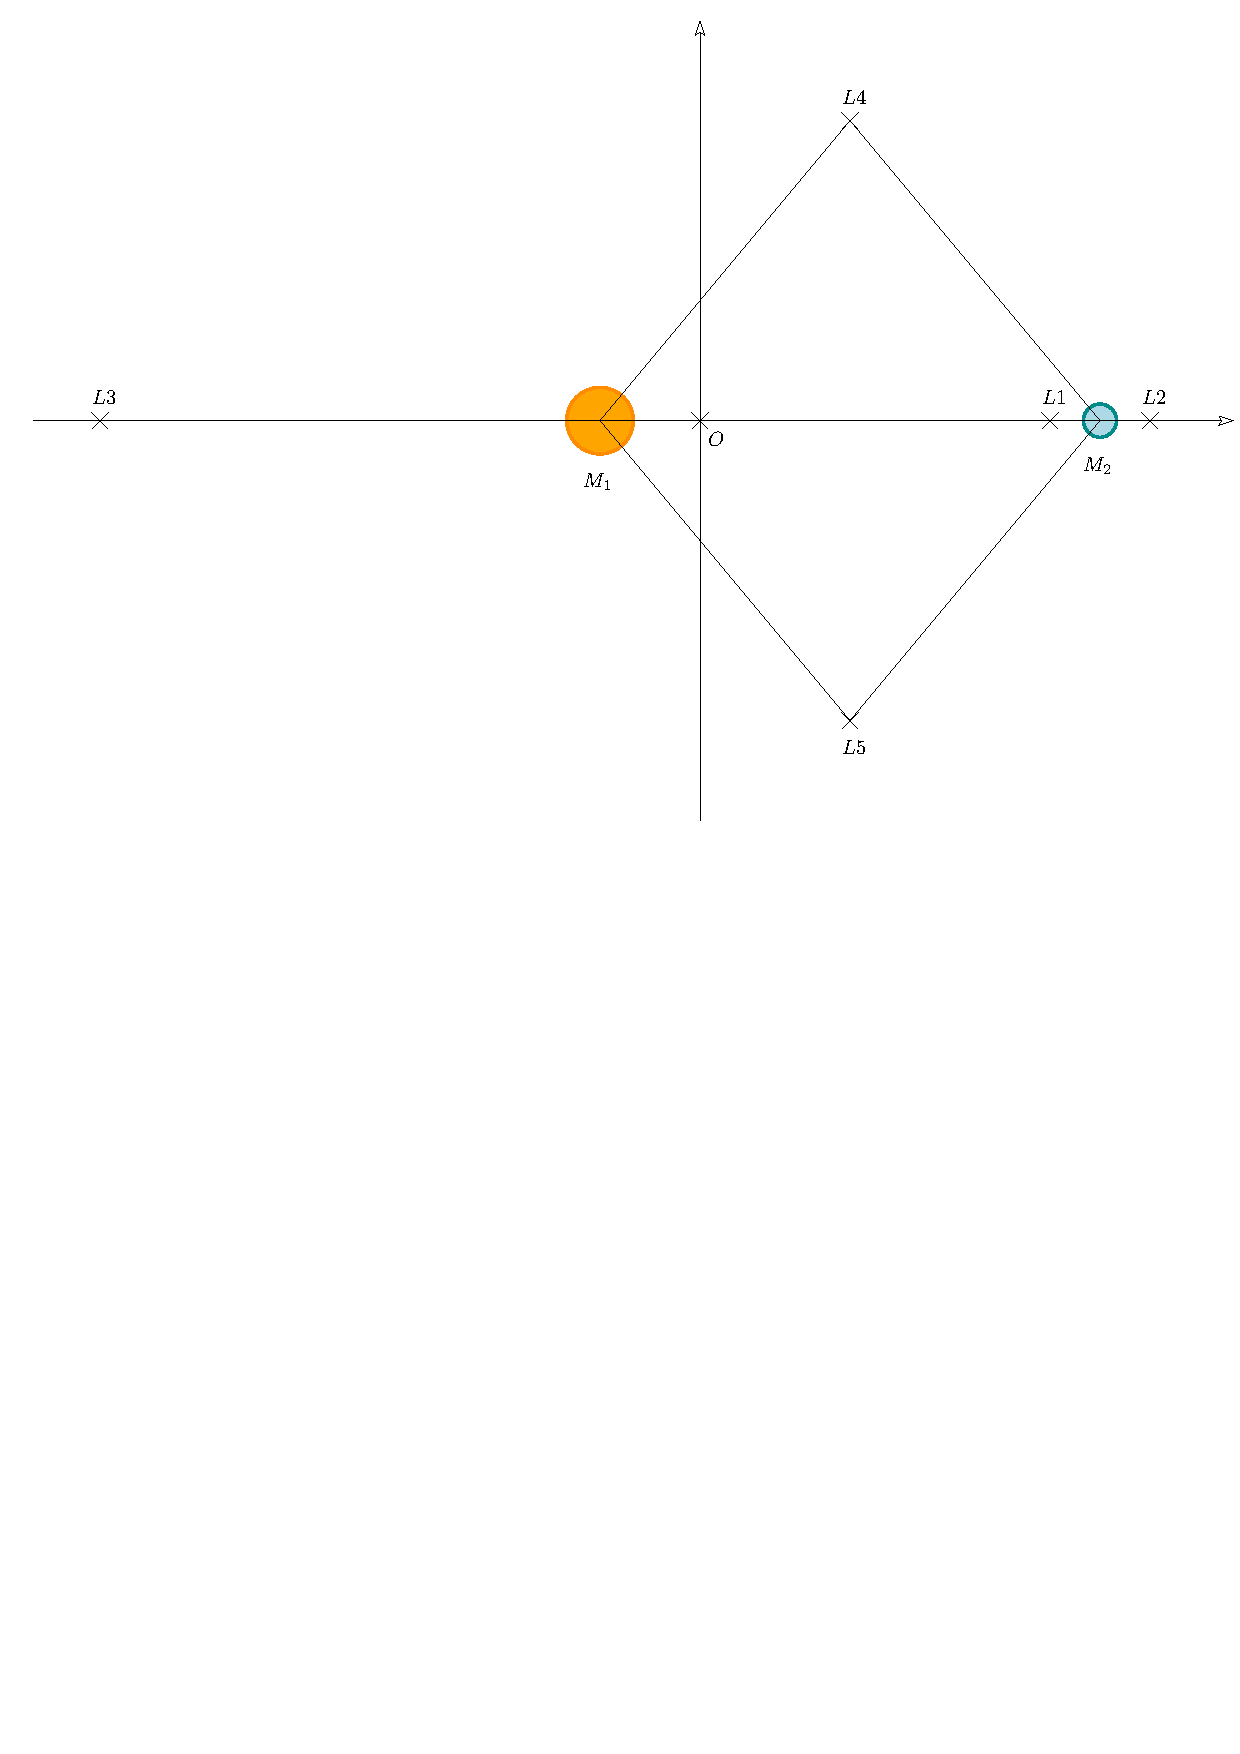
\includegraphics[width=0.8\textwidth]{ref_rng_avec_points_deq.pdf}
			\caption{Positions des points de Lagrange dans le plan d'étude.}
		\end{figure}
	\end{frame}
	
	
	\subsection{Résolution du système linéarisé}
	\begin{frame}
		\frametitle{Linéarisation des équations du mouvement}
		Les équations du mouvements sont
		\begin{equation*}
			\label{équations du mouvement}
			\begin{cases}
				\dot{x} = v_x
				\\
				\dot{y} = v_y
				\\
				\dot{v_x} = \ddot{x} = 2\omega\dot{y} - \frac{1}{m}\bar{\mathcal{U}}_x
				\\
				\dot{v_y} = \ddot{y} = - 2\omega\dot{x} - \frac{1}{m}\bar{\mathcal{U}}_y
			\end{cases}
		\end{equation*}
		Ce qui se linéarise en
		\begin{equation}
			\begin{bmatrix}
				0 & 0 & 1 & 0 \\
				0 & 0 & 0 & 1 \\
				-\frac{1}{m}\bar{U}_{xx}^i & -\frac{1}{m}\bar{U}_{xy}^i
				& 0 & 2\omega \\
				-\frac{1}{m}\bar{U}_{yx}^i & -\frac{1}{m}\bar{U}_{yy}^i
				& -2\omega & 0
			\end{bmatrix}
			=: A
		\end{equation}
		où $\bar{U}_{wz}^i = \frac{\partial ^2\bar{U}}{\partial w \partial z}(x_{L_i}, y_{L_i})$
	\end{frame}
	
	\begin{frame}
		\frametitle{Résolution}
		Le calcul du polynôme caractéristique $\chi_A$ de $A$ nous donne :
		\begin{equation*}
			A = P
			\begin{bmatrix}
				\lambda & 0 & 0 & 0 \\
				0 & -\lambda & 0 & 0 \\
				0 & 0 & i\nu & 0 \\
				0 & 0 & 0 & -i\nu
			\end{bmatrix}
			P^{-1}, \text{ avec } 
			{\footnotesize \begin{cases}
				\lambda = \omega\sqrt{1+2\sqrt{7}} \\
				\nu = \omega\sqrt{2\sqrt{7}-1}
			\end{cases}}
		\end{equation*}
		
		\pause
		On en déduit l'expression explicite des solutions dans le plan :
		{\scriptsize 		
		\begin{equation}
			\mathcal{S}_{lin}^{pos} = \{ t \to
			\begin{bmatrix}
				C_1e^{\lambda t} + C_2e^{-\lambda t} + (C_3+C_4)\cos(\nu t)
				\\
				-\sigma C_1e^{\lambda t} + \sigma C_2e^{-\lambda t} + \tau (C_3+C_4) \sin(\nu t)
			\end{bmatrix},
			(C_1,C_2,C_3,C_4) \in \mathbb{R}^3
			\}
		\end{equation}}
		
		où $\sigma > 0$ et $\tau < 0$ sont des constantes.
	\end{frame}
	
	
	\subsection{Schéma numérique pour le système non-linéaire}
	\begin{frame}
		\frametitle{Simulation de la dégénérescence autour de L1}
		\begin{figure}
			\centering
			
\includegraphics[width=0.75\linewidth]{degenerescence_L1_plots_RK4.png}
			\label{fig:instability simulation}
			\caption[width=0.75\linewidth]{Simulation numérique par schéma de Runge-Kutta 4 de la dégénérescence de l'orbite autour de L1.}
		\end{figure}
		
		
	\end{frame}
	
	
	
	
	

	
	\section[Variétés autour de L1 et L2]{Globalisation des variétés des orbites autour de L1 et L2}
	\subsection{Existence d'orbites périodiques}
	
	\begin{frame}
		\frametitle{Obtention d'une orbite}
		\begin{importantresult}{Forme générale des solutions dans l'espace de phase}
			{\scriptsize
			\begin{equation}
				\mathcal{S}_{lin} = \{ t \to
				\begin{bmatrix}
					C_1e^{\lambda t} + C_2e^{-\lambda t} + R\cos(\nu t - \varphi)
					\\
					-\sigma (C_1e^{\lambda t} - C_2e^{-\lambda t}) +  \tau R\sin(\nu t - \varphi)
					\\
					\lambda (C_1e^{\lambda t} - C_2e^{-\lambda t}) + \nu R\sin(\nu t - \varphi)
					\\
					-\lambda\sigma (C_1e^{\lambda t} + C_2e^{-\lambda t}) + \nu\tau R\cos(\nu t - \varphi)
				\end{bmatrix},
				(C_1,C_2,R,\varphi) \in \mathbb{R}^4
				\}
			\end{equation}
			}
		\end{importantresult}
		
		\bigskip
		
		\pause
		
		{\footnotesize	
		On en déduit qu'une orbite de rayon $R$ à pour condition initiale	
		$
			\begin{cases}
				x_0 = R
				\\
				y_0 = 0
				\\
				v_{x0} = 0
				\\
				v_{y0} = \nu\tau R
			\end{cases}
		$}
		
	\end{frame}
	
	\begin{frame}
		\frametitle{Optimisation numérique des caractéristiques de l'orbite}
		\begin{columns}[T]
			\column{0.4\linewidth}
			{\small Conditions initiales proposées :
			\begin{itemize}
				\item $x_0 = 1000 \: km$
				\item $y_0 = 0 \: km$
				\item $v_{x0} = 0 \: m.s^{-1}$
				\item $v_{y0} = 23,7 \: m.s^{-1}$
			\end{itemize}
		car $\nu\tau = -2,37 \cdot 10^{-5} \: s^{-1}$
		}
		
			\column{0.02\textwidth}
			\centering
			\textcolor{gray!40}{\rule{0.2pt}{0.4\textheight}}
			
			\pause
			
			\column{0.58\linewidth}
			{\small Orbite corrigée par correction itérative :}
			\begin{figure}
				\centering
				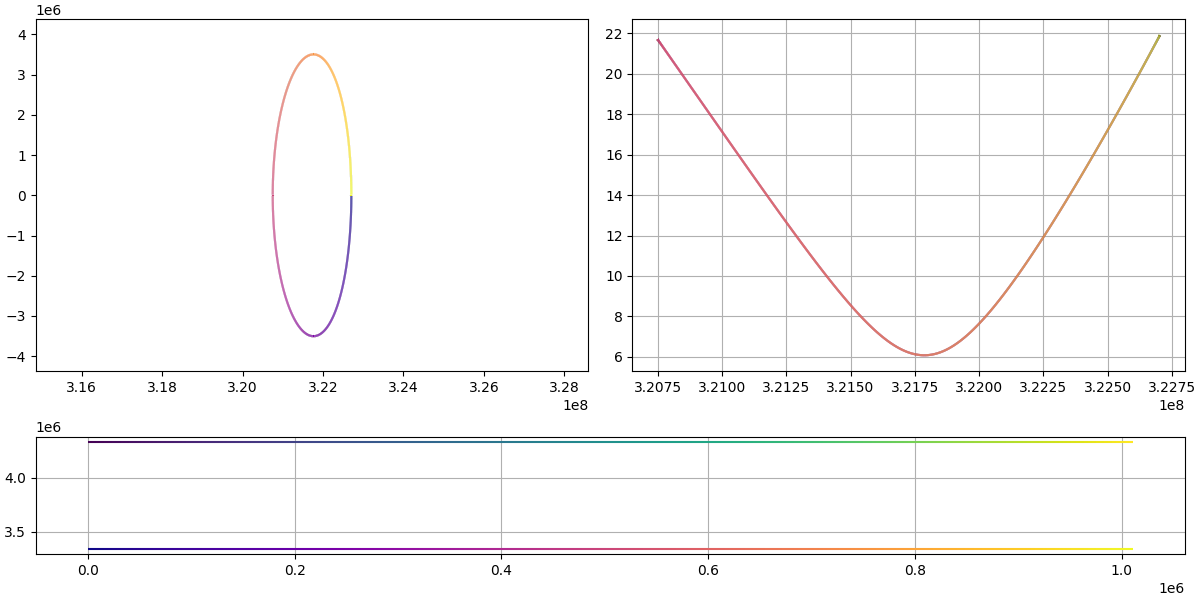
\includegraphics[width=1\linewidth]{acceptable_orbit.png}
				\caption{Simulation d'une orbite, notée $\gamma$, avec les conditions initiales $x_0 = 1000 \: km$, $y_0 = 0 \: km$, $v_{x0} = 0 \: m.s^{-1}$, et $v_{y0} = -21.898965265005835 \: m.s^{-1}$.}
			\end{figure}
		\end{columns}
	\end{frame}
	
	\begin{frame}
		\frametitle{Illustration de la correction itérative}
		\begin{figure}
			\centering
			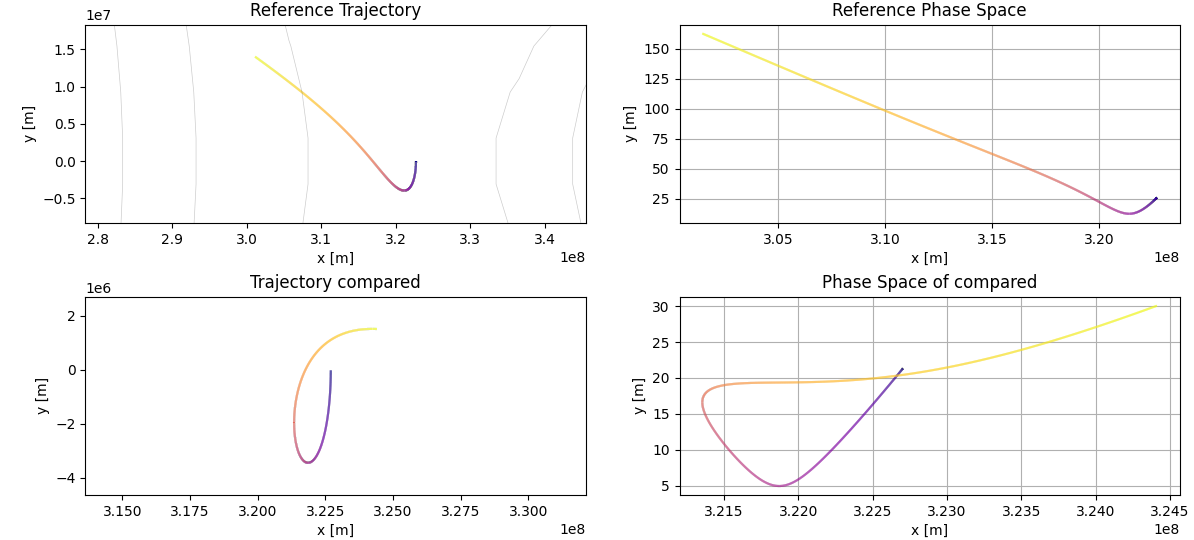
\includegraphics[width=0.85\linewidth]{iterative_correction_showcase.png}
			\caption{Illustration de la méthode de correction itérative par dichotomie (Code python en annexe \ref{py:code de correction itérative d'orbite}).}
		\end{figure}
	\end{frame}
	
	
	\subsection{Introduction à la théorie de Floquet}
	
	\begin{frame}
		\frametitle{Une petite définition...}
		{\footnotesize
		\begin{mydefinition}{Matrice fondamentale}
			Soit $(y_1,\dots,y_n)$ un système fondamentale de solutions d'une équation différentielle. Une matrice fondamentale de cette équation différentielle est l'application $t \mapsto \Phi(t)$ où $\Phi(t)$ est la matrice dont les colonnes sont les vecteurs $(y_1(t),\dots,y_n(t))$.
			
			Si $\Phi$ et $\Psi$ sont deux matrices fondamentales de la même équation différentielle, alors
			\begin{equation*}
				\exists M \in GL_n(\mathbb{C}), \Phi = \Psi M
			\end{equation*}
		\end{mydefinition}
		
		\bigskip
		
		\textit{Remarque :} Un résultat utile
		
		Si $y$ est une solution de l'équation différentielle, alors $\forall t \in \mathbb{R}, y(t) = \Phi(t)y_0$ où $\Phi$ est \textbf{la} matrice fondamentale principale.
		}
	\end{frame}
	
	\begin{frame}
		\frametitle{...et deux autres...}
		{\footnotesize
		\begin{mydefinition}{Le flot}
			On définit le flot comme l'application $ \eta :
			\begin{array}{rcl}
				\mathbb{R} \times \mathbb{R}^4 & \to & \mathbb{R}^4 \\
				(t,x_0) & \mapsto & x(t)
			\end{array}
			$ où $x$ correspond à l'unique solution au problème de Cauchy de condition initiale $x_0$.
			
			On peut remarquer qu'on a alors la relation
			\begin{equation*}
				\forall x_0 \in \mathbb{R}^4, \forall t \in \mathbb{R}, \eta(t,x_0) = \Phi(t)x_0
			\end{equation*}
		\end{mydefinition}
		\pause
		\begin{mydefinition}{Matrice de Monodromie}
			Soit une équation différentielle de la forme $X'=A(t)X$ où A est à coefficients $T$-périodiques. On appelle \textit{matrice de Monodromie} la matrice $M = \Phi(T)$ où $\Phi$ est la matrice fondamentale principale du système.
		\end{mydefinition}
		}
	\end{frame}
	
	\begin{frame}
		\frametitle{Sensibilité du système aux conditions initiales}
		{\small Le flot vérifie pour $t \in \mathbb{R}$ fixé, $x_0 \in \mathbb{R}^4$ et $\delta x_0$ une petite variation,
		\begin{equation*}
			\eta(t,x_0+\delta x_0) = \Phi(t)(x_0+\delta x_0) = \eta(t,x_0) + \Phi(t)\delta x_0 + \underset{\delta x_0 \to 0}{o}(\delta x_0)
		\end{equation*}
		\pause
		\bigskip
		dont on déduit le}
		
		\begin{importantresult}{Lien matrice de Monodromie/sensibilité aux C.I.}
			\begin{equation}
				\forall k \in \mathbb{N}^*, \delta x(kT) = M^k\delta x_0
			\end{equation}
		\end{importantresult}
	\end{frame}
	
	\subsection{Vecteurs propres de la matrice de Monodromie}
	
	\begin{frame}
		\frametitle{En quête de la Monodromie}
		{\small 
		\begin{importantresult}{Méthode numérique pour calculer $M$}
			\begin{enumerate}
				\item Calcul du linéarisé en chaque point de l'orbite $A : t \mapsto Jf(\gamma(t))$.
				\item Intégration de $\Phi(0) = I_n$ par le linéarisé le long de l'orbite, pendant une période $T$.
			\end{enumerate}
		\end{importantresult}
		}
		
		\pause
		
		\begin{columns}[T]
			\column{0.48\linewidth}
			\textbf{Linéarisé :}
			\bigskip
			{\footnotesize
			\begin{equation*}
				\begin{bmatrix}
					0 & 0 & 1 & 0 \\
					0 & 0 & 0 & 1 \\
					-\frac{\bar{U}_{xx}(\gamma(t))}{m} & -\frac{\bar{U}_{xy}(\gamma(t))}{m} & 0 & 2\omega \\
					-\frac{\bar{U}_{xy}(\gamma(t))}{m} & -\frac{\bar{U}_{yy}(\gamma(t))}{m} & -2\omega & 0
				\end{bmatrix}
			\end{equation*}
			}
			
			\column{0.02\textwidth}
			\centering
			\textcolor{gray!40}{\rule{0.2pt}{0.4\textheight}}
			\pause	
			
			\column{0.48\linewidth}
			\textbf{Orbite de référence :}
			\begin{figure}
				\centering
				
\includegraphics[width=0.7\linewidth]{acceptable_orbit_traj_only.png}
				\caption{Trajectoire de l'orbite de référence $\gamma$.}
			\end{figure}
			
		\end{columns}
		
	\end{frame}
	
	\begin{frame}
		\frametitle{Calcul numérique de $M$}
		\begin{figure}
			\centering
			{\footnotesize \begin{equation*}
				M = \begin{bmatrix} 
					1.62 \cdot 10^{3} & -2.48 \cdot 10^{2} & 1.54 \cdot 10^{8} & 7.52 \cdot 10^{7}\\
					-7.92 \cdot 10^{2} & 1.22 \cdot 10^{2} & -7.52 \cdot 10^{7} & -3.69 \cdot 10^{7}\\
					1.28 \cdot 10^{-2} & -1.96 \cdot 10^{-3} & 1.22 \cdot 10^{3} & 5.96 \cdot 10^{2}\\
					-6.01 \cdot 10^{-3} & 9.21 \cdot 10^{-4} & -5.72 \cdot 10^{2} & -2.79 \cdot 10^{2}\\
				\end{bmatrix}
			\end{equation*}
			\begin{equation*}
				\text{Sp}(M) = \{\underbrace{2.68 \cdot 10^{3}}_{=: \lambda_i}\: , \underbrace{3.74 \cdot 10^{-4}}_{=: \lambda_s}\: , 9.97 \cdot 10^{-1}\: , 1.00\}
			\end{equation*}}
			{\tiny \begin{equation*}
				P = \begin{bmatrix}
					-8.98 \cdot 10^{-1} & -8.98 \cdot 10^{-1} & -2.82 \cdot 10^{-1} & -2.84 \cdot 10^{-1}\\
					4.40 \cdot 10^{-1} & -4.40 \cdot 10^{-1} & 9.59 \cdot 10^{-1} & -9.59 \cdot 10^{-1}\\
					-7.11 \cdot 10^{-6} & 7.11 \cdot 10^{-6} & 1.55 \cdot 10^{-6} & -1.55 \cdot 10^{-6}\\
					3.34 \cdot 10^{-6} & 3.34 \cdot 10^{-6} & 6.06 \cdot 10^{-6} & 6.10 \cdot 10^{-6}\\
				\end{bmatrix}
			\end{equation*}}
			\caption{Matrice de Monodromie calculée numériquement (\textit{cf.} Annexe \ref{calcul de la matrice de monodromie}) pour l'orbite de référence $\gamma$.}
		\end{figure}
	\end{frame}
	
	\subsection{Calcul numérique des variétés}
	\begin{frame}
		\frametitle{Les directions propres}
		Sensibilités aux variations de C.I. dans une direction propre pour le linéarisé :
		\begin{equation*}
			\forall k \in \mathbb{N}^*, \delta x(kT) = \lambda^k_u x_u, \: \text{ où } u \in \{s,i\}
		\end{equation*}
		\begin{figure}
			\centering
			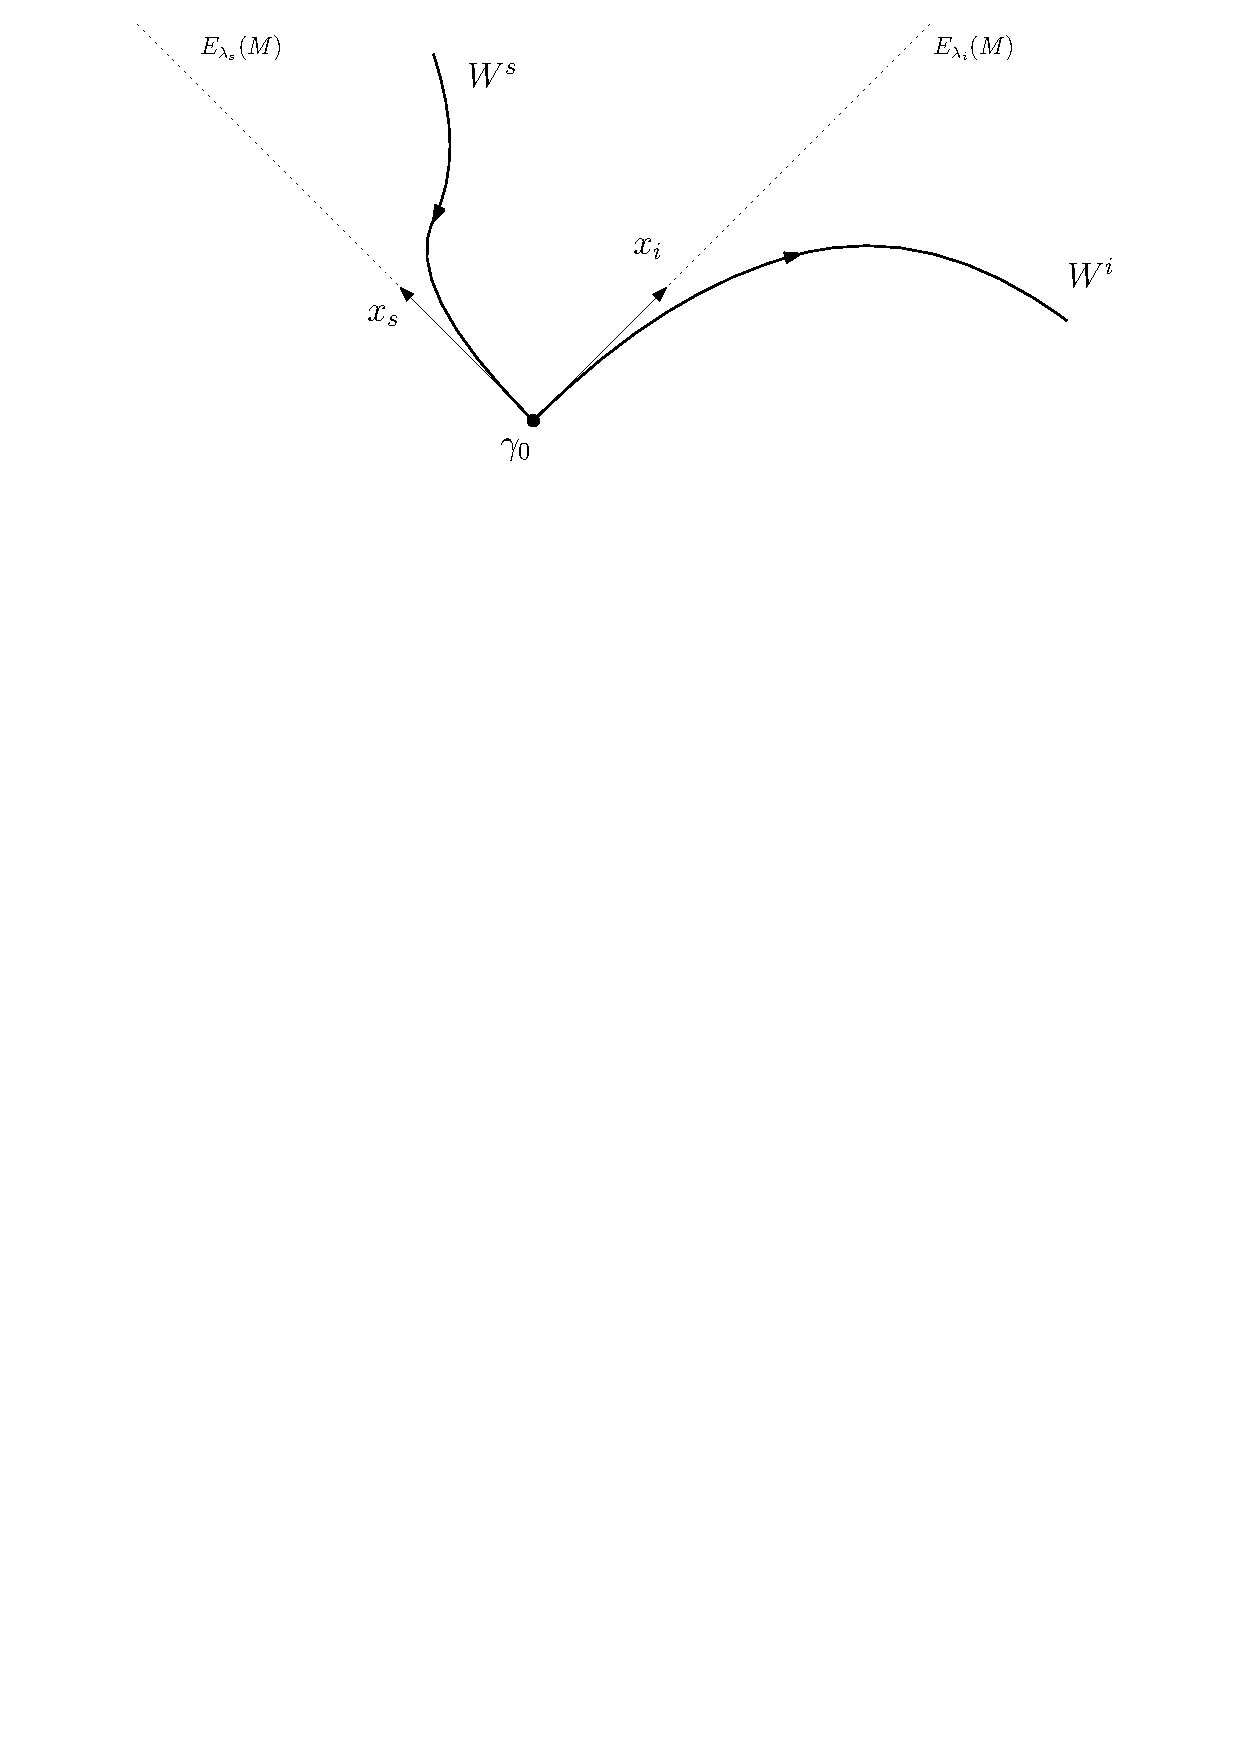
\includegraphics[width=0.8\linewidth]{illustration_varietes_lin_non_lin.pdf}
		\end{figure}
	\end{frame}
	
	\begin{frame}
		\frametitle{Calcul numérique des variétés}
		On utilise comme condition initiale $\gamma_0 \pm \varepsilon \mathcal{N} x_i$ où $\varepsilon = 10^{-6}$ et $\mathcal{N}$ est la dimensionalisation du problème pour l'espace des phases ($*$).
		
		\bigskip
		\bigskip
		
		\begin{columns}[T]
			\column{0.48\linewidth}
			\textbf{Variété instable}
			
			{\footnotesize On intègre le système non-linéaire \ref{eq du mvt} en prenant comme condition initiale celle précédente.}
			
			\pause
			
			\column{0.02\textwidth}
			\centering
			\textcolor{gray!40}{\rule{0.2pt}{0.4\textheight}}
			
			\column{0.48\linewidth}
			\textbf{Variété stable}
			
			{\footnotesize On intègre le système non-linéaire en temps décroissant. Cela revient à intégrer
			\begin{equation*}
				X' = -f(X)
			\end{equation*}
			avec la condition initiale ci-dessus.}
			
			\photosources{($*$) Dynamical Systems, the Three-Body Problem
				and Space Mission Design}
		\end{columns}
	\end{frame}
	
	\begin{frame}
		\begin{figure}
			\centering
			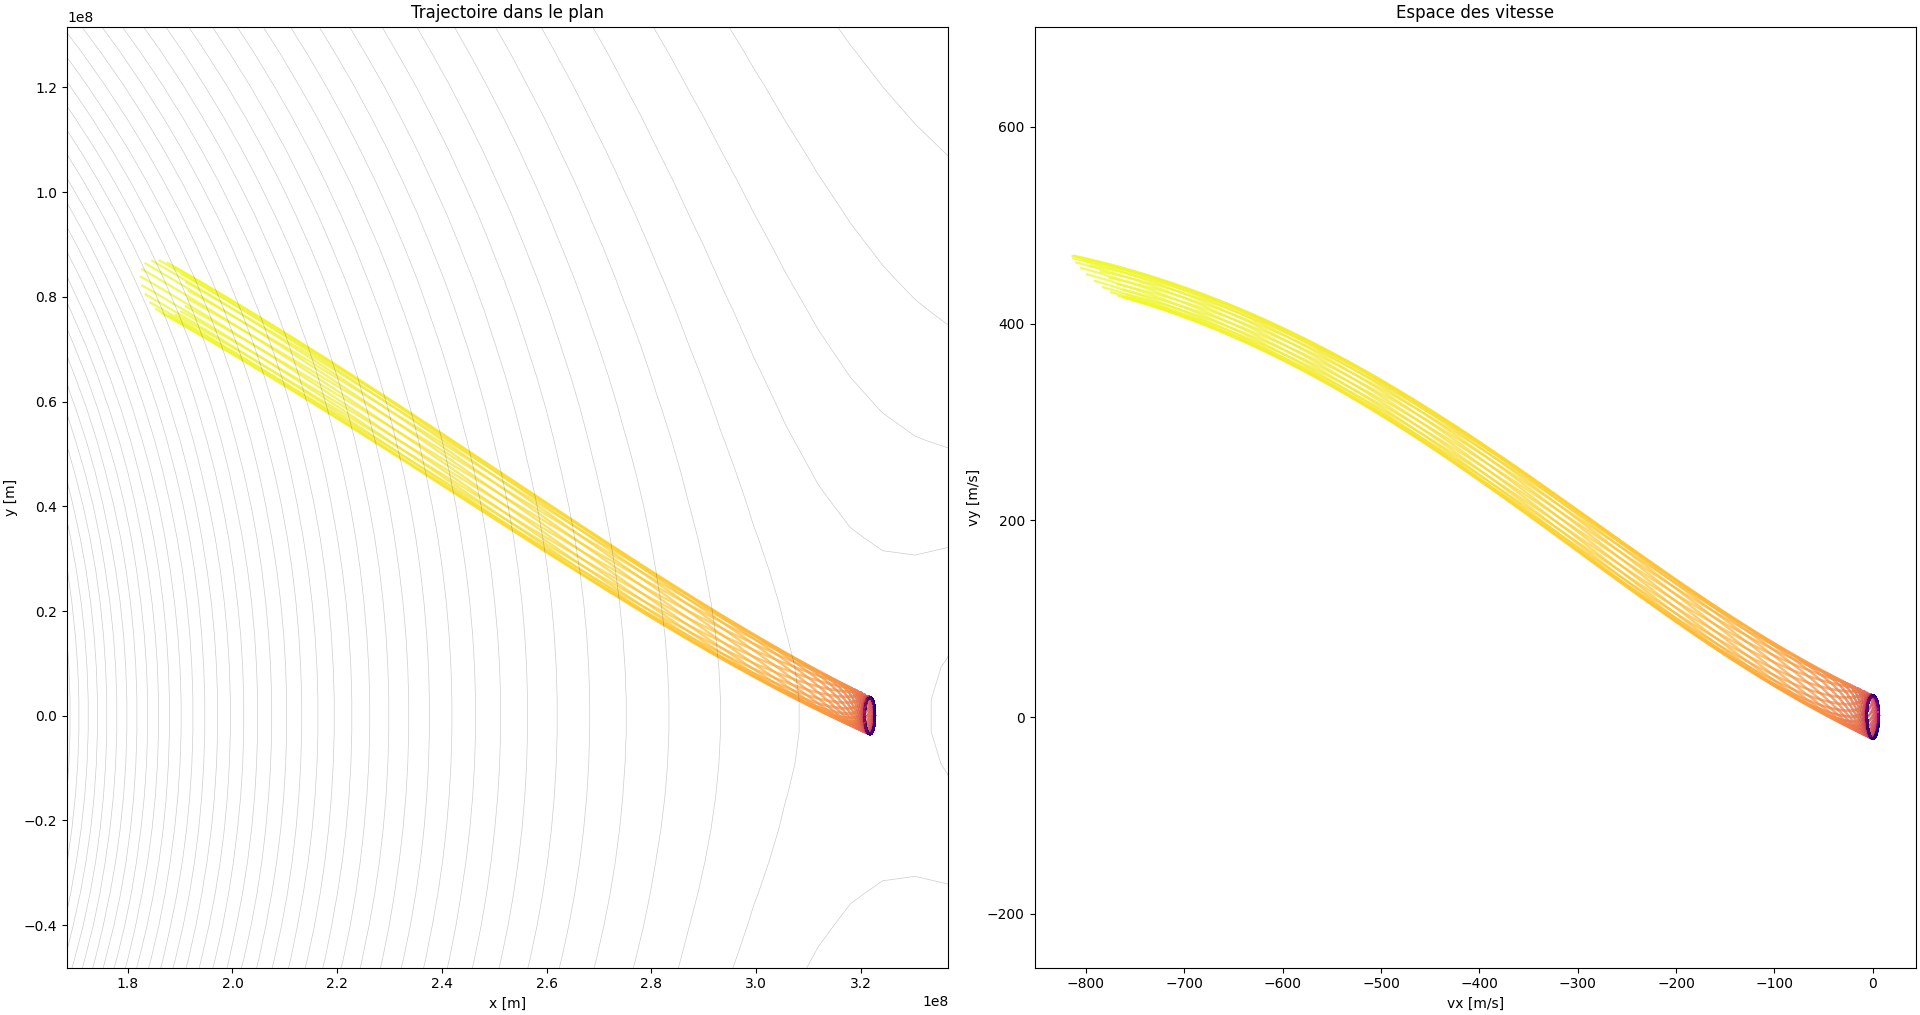
\includegraphics[width=0.9\linewidth]{variete_instable_positive_tmp}
			\caption{Projections dans le plan $(x,y)$ et dans le plan $(v_x,v_y)$ du sens positif de la variété instable de l'orbite de référence $\gamma$.}
		\end{figure}
	\end{frame}
	
	
	
	
	
	
	
	
	
	
	
	
\end{document}